\documentclass[12pt,a4paper,preprint]{elsarticle}

\usepackage[utf8]{inputenc}
\usepackage[english]{babel}
\usepackage[a4paper,left=2cm,right=2cm,top=2cm,bottom=2.7cm]{geometry}
\usepackage{amsmath,amssymb,amsfonts,amsthm,bm,graphicx,booktabs,multirow,array,tabularx,xcolor,hyperref}

\makeatletter
\def\ps@pprintTitle{%
    \let\@mkboth\markboth
    \def\@evenhead{%
        \ifnum\c@page>1
            {\footnotesize\thepage}\hfil{\footnotesize\itshape\leftmark}%
        \fi}%
    \def\@oddfoot{\footnotesize\itshape
        Preprint, \today\hfill\thepage\relax}%
    \let\@evenfoot\@oddfoot
}
\AtBeginDocument{\pagestyle{pprintTitle}}
\makeatother
\graphicspath{{figs/}}

\begin{document}
\begin{frontmatter}

\title{Acoustic geometry and sound-ray dynamics\\
in relativistic spherical accretion}

\author{Alexander V. Semyannikov}
\address{Independent Researcher \\ \textit{Email: avsemyannikov@gmail.com}}

\begin{abstract}
In analogue gravity, sound waves in a moving fluid propagate along the null geodesics of an effective curved metric, providing a controlled setup for studying horizon physics in astrophysical accretion. The relativistic acoustic metric for spherical accretion is well known and has been used in stability and quasinormal mode studies; however, the geometric optics of sound rays in the Michel flow has hitherto received little systematic attention. In the present work, the acoustic metric of a perfect fluid accreting onto a Schwarzschild black hole (the Michel flow) is constructed, and high-frequency sound rays are treated as its null geodesics. From the linearized system of continuity, Euler, and energy equations, the causal surfaces of the geometry are identified---the acoustic horizon (coinciding with the sonic point), the stationary limit surface, and the ergoregion---and a generalized Binet equation is derived, decomposing the ray deflection into Einstein, refractive, and acoustic wind contributions. The local slowdown factor allows the acoustic and vacuum Shapiro delays to be compared, the acoustic photon sphere to be localized, and the analogue Hawking scale to be linked to hydrodynamic gradients. The results for polytropic indices $\gamma=4/3$ and $5/3$ demonstrate how the thermodynamic and accretion flow parameters enter the acoustic lensing, time delay, and analogue Hawking temperature, providing a geometric foundation for future studies of finite-frequency acoustic, vortical, and entropic modes.
\end{abstract}

\begin{keyword}
acoustic metric \sep analogue gravity \sep Michel accretion \sep
Shapiro delay \sep sound rays \sep acoustic horizon \sep photon sphere \sep
Hawking temperature
\end{keyword}

\end{frontmatter}

\section{Introduction}
\label{sec:introduction}

Accretion onto black holes is a central process in high-energy astrophysics: the flow of matter onto a compact object generates electromagnetic radiation, fuels active galactic nuclei, and provides one of the few laboratories where strong gravity can be studied observationally~\cite{ShapiroSL_TeukolskySA_BlackHolesWhiteDwarfsAndNeutronStarsThePhysicsOfCompactObjects_2004}. Alongside the geometry of spacetime itself, the \emph{hydrodynamics} of the accreting fluid sustains an independent causal structure for sound. In a moving medium, acoustic perturbations propagate as if they resided on an effective Lorentzian geometry---the \emph{acoustic metric}---whose null cones define sound horizons, ergoregions, and, in suitable regimes, analogues of Hawking radiation~\cite{UnruhWG_ExperimentalBlackHoleEvaporation_1981, VisserM_AcousticBlackHolesHorizonsErgospheresAndHawkingRadiation_1998, BarceloC_LiberatiS_VisserM_AnalogueGravity_2011}. This analogue gravity correspondence links the theory of wave equations in curved spacetime with the astrophysics of transonic accretion.

The classical Newtonian description of stationary spherical accretion is due to Bondi~\cite{BondiH_OnSphericallySymmetricalAccretion_1953}. Its general-relativistic counterpart on a Schwarzschild background---the Michel flow~\cite{MichelFC_AccretionOfMatterByCondensedObjects_1972}---is a stationary, spherically symmetric, adiabatic solution that passes through the sonic point and becomes supersonic near the event horizon. Linear acoustic perturbations of such flows are described by a scalar wave equation on an effective metric constructed from the background spacetime, the fluid 4-velocity, and the local speed of sound. A version of this construction is present in Moncrief's analysis of the stability of spherical accretion onto a Schwarzschild black hole~\cite{MoncriefV_StabilityOfStationarySphericalAccretionOntoASchwarzschildBlackHole_1980}; relativistic acoustic geometry was subsequently systematized by Bilic~\cite{BilicN_RelativisticAcousticGeometry_1999} and placed in the broader context of analogue gravity by Visser~\cite{VisserM_AcousticBlackHolesHorizonsErgospheresAndHawkingRadiation_1998} and Barcelo, Liberati, and Visser~\cite{BarceloC_LiberatiS_VisserM_AnalogueGravity_2011}.

In this setup, a significant portion of the work on Michel accretion focuses on the wave equation: global stability outside the sonic horizon, energy estimates, and the spectrum of quasinormal acoustic oscillations~\cite{MoncriefV_StabilityOfStationarySphericalAccretionOntoASchwarzschildBlackHole_1980, ChaverraE_MoralesMD_SarbachO_QuasinormalAcousticOscillationsInTheMichelFlow_2015}, while analogue Hawking radiation has been reinterpreted as a tunneling process~\cite{JangidN_RayAK_AcousticHawkingRadiationAsATunnellingEffectInMichelAccretion_2026}. A complementary line of work expresses the acoustic surface gravity and analogue Hawking temperature directly in terms of accretion variables for relativistic flows~\cite{DasTK_BilicN_DasguptaS_BlackHoleAccretionDiscAsAnAnalogueGravityModel_2007, TarafdarP_DasTK_GeometricConfigurationOfMatterForAxiallySymmetricBackgroundFlowsInTheSchwarzschildMetric_2013, ShaikhMA_FirdousiI_DasTK_RelativisticSonicGeometryForIsothermalAccretionInTheSchwarzschildMetric_2017}. The ray properties of acoustic metrics have been studied predominantly in other analogue setups~\cite{ToshmatovB_AhmedovB_StuchlikZ_PhononMotionAround21DimensionalAcousticBlackHole_2023, BalaliAE_MarraniA_LenseThirringAcousticBlackHolesShadowsAndLight_2025, VieiraHS_DestounisK_KokkotasKD_AnalogSchwarzschildBlackHolesOfBoseEinsteinCondensatesInACavityQuasinormalModesAndQuasiboundStates_2023, PalK_PalK_SarkarT_AnalogueMetricInABlackBounceBackground_2022}. These studies establish the acoustic geometry of Michel accretion as a genuine astrophysical analogue black hole, yet they do not provide a unified geometric-optics phenomenology of \emph{sound rays} for the relativistic adiabatic Michel flow.

In vacuum theory, null geodesics underpin gravitational lensing, the photon sphere, and the Shapiro time delay~\cite{ShapiroII_FourthTestOfGeneralRelativity_1964}. For relativistic Michel accretion, these ray-level questions---the forces deflecting a sound ray, the acoustic Shapiro delay, the shift of the acoustic photon sphere, and the surface gravity of the sound horizon---have not previously been synthesized into a single quantitative picture linked to the flow thermodynamics.

In the present work, the relativistic acoustic metric of a perfect fluid in stationary Michel accretion onto a Schwarzschild black hole is constructed, and its high-frequency sound rays are studied as null geodesics of the effective spacetime. Specifically:
\begin{itemize}
    \item the acoustic horizon, stationary limit surface, and ergoregion are identified, and the coincidence of the horizon with the Michel sonic point is verified;
    \item a generalized Binet equation is derived, decomposing the ray deflection into Einstein, refractive, and acoustic wind forces, which are numerically evaluated for polytropic indices $\gamma=4/3$ and $5/3$;
    \item a local slowdown factor $n_{\pm}=f/|v_{\pm}|$ is introduced and used to compare the acoustic and vacuum Shapiro delays along radial rays;
    \item the acoustic photon sphere is localized, the associated capture barrier is described, and the surface gravity of the sound horizon is expressed through hydrodynamic gradients.
\end{itemize}

\section{Relativistic fluid and acoustic perturbations}
\label{sec:fluid}

The thermodynamic and hydrodynamic elements required for the definition of the acoustic metric are summarized below. Throughout the work, the metric signature $\mathfrak{s}=(-,+,+,+)$ is used, so that the fluid 4-velocity satisfies
\begin{equation}
    u_{\mu} u^{\mu} = -1.
    \label{eq:four-velocity-norm}
\end{equation}
All quantities are dimensionless: spacetime coordinates are measured in units of the gravitational radius $r_{\mathrm{g}}=2GM/c^{2}$, the 4-velocity and sound speed in units of $c$, and the thermodynamic variables are normalized to their asymptotic rest scales~\cite{MichelFC_AccretionOfMatterByCondensedObjects_1972, MoncriefV_StabilityOfStationarySphericalAccretionOntoASchwarzschildBlackHole_1980}. Orthogonal projections onto the fluid rest frame are performed using
\begin{equation}
    \Delta^{\mu}_{\nu} = \delta^{\mu}_{\nu} + u^{\mu} u_{\nu}.
    \label{eq:projection-tensor}
\end{equation}

\subsection{Thermodynamics of a perfect fluid}

The medium is modeled as a perfect fluid in local thermodynamic equilibrium. The dimensionless specific enthalpy is given by
\begin{equation}
    h = \frac{p + \epsilon}{n},
    \label{eq:specific-enthalpy}
\end{equation}
where $p$, $\epsilon$, and $n$ are the dimensionless pressure, energy density, and baryon number density. The first law of thermodynamics,
\begin{equation}
    \mathrm{d}h = T\,\mathrm{d}S + n^{-1}\,\mathrm{d}p,
    \label{eq:first-law-thermodynamics}
\end{equation}
for an adiabatic flow ($S=\mathrm{const}$) reduces to
\begin{equation}
    \mathrm{d}p = n\,\mathrm{d}h.
    \label{eq:adiabatic-relation}
\end{equation}
Together with~\eqref{eq:specific-enthalpy}, this yields the identity $\mathrm{d}\epsilon = h\,\mathrm{d}n$.

The local speed of sound is defined by the isentropic derivative
\begin{equation}
    a^{2}
    =
    \Bigl(\frac{\partial p}{\partial\epsilon}\Bigr)_{S}
    =
    \frac{1}{h}\,\frac{\mathrm{d}p}{\mathrm{d}n}.
    \label{eq:sound-speed-def}
\end{equation}
The thermodynamics is closed by a polytropic equation of state $p = K n^{\gamma}$. Integration of~\eqref{eq:adiabatic-relation} yields
\begin{equation}
    h = 1 + \frac{\gamma K}{\gamma-1}\, n^{\gamma-1},
    \label{eq:enthalpy-polytropic}
\end{equation}
and substitution into~\eqref{eq:sound-speed-def} gives
\begin{equation}
    a^{2}
    =
    \frac{K\gamma\, n^{\gamma-1}}
         {1 + \dfrac{\gamma K}{\gamma-1}\, n^{\gamma-1}}.
    \label{eq:sound-speed-polytropic}
\end{equation}
In the cold non-relativistic limit $h\to 1$, the Newtonian relation $a^{2}\approx K\gamma n^{\gamma-1}$ is recovered. In the ultra-relativistic limit $n\to\infty$, a universal bound $a^{2}\to\gamma-1$ arises; causality ($a^{2}\le 1$) requires $\gamma\le 2$.

For subsequent use, the conformal factor of the acoustic metric is recorded in terms of the local sound speed:
\begin{equation}
    \Omega^{2} 
    = \frac{n}{h} 
    \quad\Longrightarrow\quad \Omega^{2}
    = C\, a^{\frac{2}{\gamma-1}}
    \Biggl(
        \frac{\gamma-1}{\gamma-1-a^{2}}
    \Biggr)^{\frac{2-\gamma}{\gamma-1}},
    \label{eq:conformal-factor}
\end{equation}
where $C=(K\gamma)^{-1/(\gamma-1)}$ is fixed by the flow entropy. The global constant $C$ cancels in the null interval condition and does not affect the kinematics of sound rays.

\subsection{Hydrodynamic equations}

Particle number conservation is expressed by the continuity equation
\begin{equation}
    \nabla_{\mu}\bigl(n\, u^{\mu}\bigr) = 0.
    \label{eq:continuity-equation}
\end{equation}
The covariant conservation of the perfect fluid stress-energy tensor,
\begin{equation}
    T^{\mu}_{\nu} = nh\, u^{\mu} u_{\nu} + p\,\delta^{\mu}_{\nu},
    \qquad
    \nabla_{\mu} T^{\mu}_{\nu} = 0,
    \label{eq:stress-energy-tensor}
\end{equation}
together with~\eqref{eq:continuity-equation} and~\eqref{eq:adiabatic-relation}, leads to the relativistic Euler equation
\begin{equation}
    h\, u^{\mu}\nabla_{\mu} u_{\nu}
    +
    \Delta^{\mu}_{\nu}\nabla_{\mu} h
    = 0.
    \label{eq:euler-enthalpy}
\end{equation}
Introducing the relativistic vorticity 2-form
\begin{equation}
    \omega_{\mu\nu}
    \equiv
    \partial_{\mu}\bigl(h u_{\nu}\bigr)
    -
    \partial_{\nu}\bigl(h u_{\mu}\bigr)
    \label{eq:vorticity-2form}
\end{equation}
and allowing for a non-zero entropy gradient, Eq.~\eqref{eq:euler-enthalpy} is rewritten in the Lichnerowicz--Crocco form:
\begin{equation}
    u^{\mu}\omega_{\mu\nu} = T\,\partial_{\nu} S.
    \label{eq:euler-vorticity}
\end{equation}
The projection of $\nabla_{\mu}T^{\mu}_{\nu}=0$ along the flow is equivalent to entropy advection,
\begin{equation}
    u^{\mu}\partial_{\mu} S = 0.
    \label{eq:entropy-advection}
\end{equation}
The triad~\eqref{eq:continuity-equation}--\eqref{eq:euler-vorticity}--\eqref{eq:entropy-advection} closes the perfect fluid dynamics. Upon linearization, it splits the perturbation spectrum into three families: acoustic, vortical, and entropic modes~\cite{MoncriefV_StabilityOfStationarySphericalAccretionOntoASchwarzschildBlackHole_1980}.

\subsection{Linear perturbations and the acoustic wave equation}

Each field is represented as a background value plus a first-order perturbation,
\begin{equation}
    h\to h+\delta h,\quad
    u^{\mu}\to u^{\mu}+\delta u^{\mu},\quad
    n\to n+\delta n,\quad
    S\to S+\delta S.
    \label{eq:perturbation-expansion}
\end{equation}
The density and enthalpy perturbations are related by
\begin{equation}
    \delta n = \frac{n}{a^{2} h}\,\delta h,
    \label{eq:density-enthalpy-perturbation}
\end{equation}
and the linearization of~\eqref{eq:four-velocity-norm} imposes the orthogonality condition $u_{\mu}\delta u^{\mu}=0$. The linearized continuity equation then takes the form
\begin{equation}
    \nabla_{\mu}
    \Biggl(
        n
        \Biggl[
            \delta u^{\mu}
            +
            \frac{u^{\mu}}{h a^{2}}\,\delta h
        \Biggr]
    \Biggr)
    = 0.
    \label{eq:linearized-continuity}
\end{equation}

The background is assumed to be homoentropic ($\nabla_{\mu}S=0$) and irrotational ($\omega_{\mu\nu}=0$). Defining the perturbed generalized momentum
\begin{equation}
    w_{\mu}
    \equiv
    \delta\bigl(h u_{\mu}\bigr)
    =
    h\,\delta u_{\mu} + u_{\mu}\,\delta h
    \label{eq:perturbed-momentum}
\end{equation}
and its vorticity $\delta\omega_{\mu\nu}=\partial_{\mu}w_{\nu}-\partial_{\nu}w_{\mu}$, the linearized Euler equation is written as
\begin{equation}
    u^{\mu}\,\delta\omega_{\mu\nu} = T\,\partial_{\nu}\delta S.
    \label{eq:linearized-euler}
\end{equation}
For acoustic modes ($\delta S=0$, $\delta\omega_{\mu\nu}=0$), $w_{\mu}=\partial_{\mu}\delta\psi$ holds, expressing the hydrodynamic fields through a scalar potential:
\begin{equation}
    h\,\delta u_{\mu} + u_{\mu}\,\delta h = \partial_{\mu}\delta\psi.
    \label{eq:velocity-potential-def}
\end{equation}
Contraction with $u^{\mu}$ yields
\begin{equation}
    \delta h = -\,u^{\mu}\partial_{\mu}\delta\psi,
    \label{eq:enthalpy-potential-relation}
\end{equation}
and the projector~\eqref{eq:projection-tensor} leads to
\begin{equation}
    h\,\delta u_{\mu}
    =
    \Delta^{\nu}_{\mu}\,\partial_{\nu}\delta\psi.
    \label{eq:velocity-potential-gradient}
\end{equation}
Substitution of~\eqref{eq:enthalpy-potential-relation} and~\eqref{eq:velocity-potential-gradient} into~\eqref{eq:linearized-continuity} yields the wave equation
\begin{equation}
    \nabla_{\mu}\bigl(\mathcal{G}^{\mu\nu}\partial_{\nu}\delta\psi\bigr) = 0,
    \label{eq:wave-equation}
\end{equation}
in which the contravariant acoustic metric has the form
\begin{equation}
    \mathcal{G}^{\mu\nu} = \Omega^{2}\,\eta^{\mu\nu},
    \qquad
    \eta^{\mu\nu} = g^{\mu\nu} + \alpha\, u^{\mu} u^{\nu},
    \label{eq:acoustic-metric-tensor}
\end{equation}
with the drag parameter $\alpha=1-a^{-2}$. The covariant counterpart is written as
\begin{equation}
    \mathcal{G}_{\mu\nu} = \Omega^{-2}\,\eta_{\mu\nu},
    \qquad
    \eta_{\mu\nu} = g_{\mu\nu} - \beta\, u_{\mu} u_{\nu},
    \label{eq:covariant-acoustic-metric-tensor}
\end{equation}
where $\beta = a^{2}-1$. The construction~\eqref{eq:acoustic-metric-tensor}--\eqref{eq:covariant-acoustic-metric-tensor} represents the relativistic acoustic geometry of Bilic~\cite{BilicN_RelativisticAcousticGeometry_1999}. High-frequency sound rays are the null geodesics of $\mathcal{G}_{\mu\nu}$.

\section{Acoustic geometry of Michel accretion}
\label{sec:acoustic-geometry}

The acoustic metric is now specialized to stationary, spherically symmetric, adiabatic accretion onto a Schwarzschild black hole---the Michel flow~\cite{MichelFC_AccretionOfMatterByCondensedObjects_1972}.

\subsection{Schwarzschild background spacetime}

The background interval is written as
\begin{equation}
    \mathrm{d}s^{2}
    =
    -f\,\mathrm{d}t^{2}
    +
    f^{-1}\,\mathrm{d}r^{2}
    +
    r^{2}\bigl(\mathrm{d}\theta^{2}+\sin^{2}\!\theta\,\mathrm{d}\phi^{2}\bigr),
    \label{eq:schwarzschild-metric}
\end{equation}
with the dimensionless lapse function
\begin{equation}
    f = 1 - r^{-1}.
    \label{eq:lapse-function}
\end{equation}
In matrix notation,
\begin{equation}
    g^{\mu\nu}
    =
    \begin{pmatrix}
        -f^{-1} & 0 & 0 & 0 \\
        0 & f & 0 & 0 \\
        0 & 0 & r^{-2} & 0 \\
        0 & 0 & 0 & r^{-2}\sin^{-2}\!\theta
    \end{pmatrix},
    \qquad
    g_{\mu\nu}
    =
    \begin{pmatrix}
        -f & 0 & 0 & 0 \\
        0 & f^{-1} & 0 & 0 \\
        0 & 0 & r^{2} & 0 \\
        0 & 0 & 0 & r^{2}\sin^{2}\!\theta
    \end{pmatrix}.
    \label{eq:schwarzschild-metric-matrix}
\end{equation}
By virtue of stationarity and spherical symmetry, every background scalar depends only on $r$. Writing
\begin{equation}
    u^{\mu} = (\vartheta,\,\upsilon,\,0,\,0),
    \label{eq:four-velocity-schwarzschild}
\end{equation}
the covariant components $u_{\mu}=(-f\vartheta,\,f^{-1}\upsilon,\,0,\,0)$ are obtained, and the normalization~\eqref{eq:four-velocity-norm} takes the form
\begin{equation}
    -u_{t} = f\vartheta = \sqrt{f+\upsilon^{2}},
    \label{eq:four-velocity-norm-schwarzschild}
\end{equation}
linking the temporal component to the radial 3-velocity of the flow. The physical velocity measured by a static observer,
\begin{equation}
    V = \frac{|\upsilon|}{\sqrt{f+\upsilon^{2}}},
    \label{eq:physical-velocity}
\end{equation}
enters the Mach number $\mathcal{M}=V/a$.

The Michel background is fixed by two integrals of motion: continuity gives the baryon flux $r^{2} n\,\upsilon=\mathrm{const}$ ($\upsilon<0$ for accretion), and the adiabatic projection integrates to the relativistic Bernoulli integral
\begin{equation}
    h\sqrt{f+\upsilon^{2}} = h_{\infty}.
    \label{eq:michel-bernoulli}
\end{equation}
Together with the polytropic closure, these relations determine the profiles $\upsilon(r)$, $a(r)$, and $n(r)$~\cite{MichelFC_AccretionOfMatterByCondensedObjects_1972, ShapiroSL_TeukolskySA_BlackHolesWhiteDwarfsAndNeutronStarsThePhysicsOfCompactObjects_2004}.

\subsection{Acoustic metric tensor}

Substituting~\eqref{eq:schwarzschild-metric-matrix} and~\eqref{eq:four-velocity-schwarzschild} into the covariant core~\eqref{eq:covariant-acoustic-metric-tensor} yields
\begin{equation}
    \eta_{\mu\nu}
    =
    \begin{pmatrix}
        -f\bigl(1+\beta f\vartheta^{2}\bigr) &
        \beta\vartheta\upsilon & 0 & 0 \\
        \beta\vartheta\upsilon &
        f^{-1}\bigl(1-\beta f^{-1}\upsilon^{2}\bigr) & 0 & 0 \\
        0 & 0 & r^{2} & 0 \\
        0 & 0 & 0 & r^{2}\sin^{2}\!\theta
    \end{pmatrix}.
    \label{eq:eta-covariant-matrix}
\end{equation}
The full covariant acoustic metric is defined as $\mathcal{G}_{\mu\nu}=\Omega^{-2}\eta_{\mu\nu}$. The corresponding contravariant core is written as
\begin{equation}
    \eta^{\mu\nu}
    =
    \begin{pmatrix}
        -f^{-1}+\alpha\vartheta^{2} &
        \alpha\vartheta\upsilon & 0 & 0 \\
        \alpha\vartheta\upsilon &
        f+\alpha\upsilon^{2} & 0 & 0 \\
        0 & 0 & r^{-2} & 0 \\
        0 & 0 & 0 & r^{-2}\sin^{-2}\!\theta
    \end{pmatrix}.
    \label{eq:eta-contravariant-matrix}
\end{equation}
Since sound rays are null geodesics of $\mathcal{G}_{\mu\nu}$, they are invariant under conformal rescalings:
\begin{equation}
    \mathcal{G}_{\mu\nu}k^{\mu}k^{\nu}=0 \quad\Longrightarrow\quad \eta_{\mu\nu}k^{\mu}k^{\nu} = 0.
    \label{eq:acoustic-null-condition}
\end{equation}
The geometry of the acoustic light cone is entirely fixed by the core $\eta_{\mu\nu}$.

\subsection{Acoustic horizon, stationary limit, and ergoregion}

The acoustic event horizon $r=r_{\mathrm{a}}$ constitutes a one-way membrane for sound and forms where the flow becomes sonic or supersonic, which is equivalent to the vanishing of the radial core component:
\begin{equation}
    \eta^{rr}(r_{\mathrm{a}}) = 0
    \quad\Longrightarrow\quad
    r_{\mathrm{a}}
    =
    \bigl[1 + \alpha(r_{\mathrm{a}})\,\upsilon^{2}(r_{\mathrm{a}})\bigr]^{-1}.
    \label{eq:acoustic-horizon-def}
\end{equation}
For $r<r_{\mathrm{a}}$, all characteristics of the wave equation are directed inward.

The acoustic stationary limit surface $r=r_{\mathrm{asl}}$ is defined by the vanishing of the temporal core component,
\begin{equation}
    \eta^{tt}(r_{\mathrm{asl}}) = 0
    \quad\Longrightarrow\quad
    r_{\mathrm{asl}}
    =
    \frac{\alpha(r_{\mathrm{asl}})\,\vartheta^{2}(r_{\mathrm{asl}})}
         {\alpha(r_{\mathrm{asl}})\,\vartheta^{2}(r_{\mathrm{asl}})-1}.
    \label{eq:stationary-limit-def}
\end{equation}
Inside $r<r_{\mathrm{asl}}$, a stationary acoustic mode cannot exist. Equating~\eqref{eq:acoustic-horizon-def} and~\eqref{eq:stationary-limit-def} would require $a^{2}<0$, which is impossible for a stable medium. Consequently, the two surfaces never coincide, $r_{\mathrm{a}} \neq r_{\mathrm{asl}}$, and the finite shell between them constitutes the acoustic ergoregion~\cite{VisserM_AcousticBlackHolesHorizonsErgospheresAndHawkingRadiation_1998, BilicN_RelativisticAcousticGeometry_1999}.

A key structural fact of Michel accretion is the exact coincidence of the acoustic horizon with the sonic critical point of the background flow. A smooth transonic transition through $r=r_{\mathrm{c}}$ requires the simultaneous vanishing of the numerator and denominator of the radial gradient equation~\cite{ShapiroSL_TeukolskySA_BlackHolesWhiteDwarfsAndNeutronStarsThePhysicsOfCompactObjects_2004}, leading to the standard critical point conditions:
\begin{equation}
    \upsilon^{2}_{\mathrm{c}} = \frac{1}{4r_{\mathrm{c}}},
    \qquad
    a^{2}_{\mathrm{c}}
    =
    \frac{1}{4r_{\mathrm{c}}-3}
    =
    \frac{\upsilon^{2}_{\mathrm{c}}}{1-3\upsilon^{2}_{\mathrm{c}}}.
    \label{eq:michel-sonic}
\end{equation}
Substituting these values into $\eta^{rr}$ from~\eqref{eq:eta-contravariant-matrix} gives
\begin{equation}
    1 - a^{-2}_{\mathrm{c}}
    =
    4(1-r_{\mathrm{c}}),
    \qquad
    \bigl(1-a^{-2}_{\mathrm{c}}\bigr)\upsilon^{2}_{\mathrm{c}}
    =
    -f_{\mathrm{c}},
\end{equation}
from which it follows that
\begin{equation}
    \eta^{rr}(r_{\mathrm{c}}) = f_{\mathrm{c}} - f_{\mathrm{c}} = 0.
    \label{eq:sonic-is-horizon}
\end{equation}
Therefore, $r_{\mathrm{a}}=r_{\mathrm{c}}$: the surface where the accretion flow becomes sonic \emph{is} the acoustic event horizon. The shell $1<r<r_{\mathrm{a}}$ is supersonic ($\eta^{rr}<0$) and terminates at the gravitational horizon $r=1$.

The Bernoulli integral~\eqref{eq:michel-bernoulli} links $a_{\infty}$ to the horizon radius $r_{\mathrm{a}}$; typical values are presented in Table~\ref{tab:sonic-point}. The numerical results rely on background profiles obtained by integrating inward from a large radius. The acoustic photon sphere $r_{\mathrm{aph}}$ is found as the maximum of the capture barrier $U(r)=a^{2}\eta^{rr}/r^{2}$.

\section{Sound-ray dynamics}
\label{sec:rays}

In the high-frequency limit, acoustic perturbations propagate along the null geodesics of $\mathcal{G}_{\mu\nu}$, which represent the acoustic analogue of light rays in vacuum~\cite{VisserM_AcousticBlackHolesHorizonsErgospheresAndHawkingRadiation_1998, BarceloC_LiberatiS_VisserM_AnalogueGravity_2011}.

\subsection{Null geodesics and conserved quantities}

The stationarity and spherical symmetry of the Michel background provide two Killing vectors, $\partial_{t}$ and $\partial_{\phi}$, which endow each sound ray with conserved energy and angular momentum. The rays themselves are null geodesics of the acoustic metric,
\begin{equation}
    \frac{\mathrm{d}^{2}x^{\mu}}{\mathrm{d}\lambda^{2}}
    +
    \Gamma^{\mu}_{\alpha\beta}
    \frac{\mathrm{d}x^{\alpha}}{\mathrm{d}\lambda}
    \frac{\mathrm{d}x^{\beta}}{\mathrm{d}\lambda}
    = 0,
    \label{eq:geodesic-equation}
\end{equation}
with the wave vector $k^{\mu}=\mathrm{d}x^{\mu}/\mathrm{d}\lambda$. The stationarity of $\mathcal{G}_{\mu\nu}$ yields the Killing-conserved energy
\begin{equation}
    k_{t} = \mathcal{G}_{t\mu}k^{\mu} = -E = \mathrm{const},
    \label{eq:energy-conservation}
\end{equation}
where the minus sign follows from the signature~\eqref{eq:four-velocity-norm}. Since $\mathcal{G}_{rt}\neq 0$,
\begin{equation}
    \frac{\mathrm{d}t}{\mathrm{d}\lambda}
    =
    -\frac{1}{\mathcal{G}_{tt}}
    \Biggl(
        E + \mathcal{G}_{rt}\,\frac{\mathrm{d}r}{\mathrm{d}\lambda}
    \Biggr),
    \label{eq:time-coordinate-derivative}
\end{equation}
the coordinate time along the ray is rigidly tied to its radial motion: the inflowing medium drags the ray forward in $t$, serving as the acoustic analogue of frame dragging.

The second Killing vector, $\partial_{\phi}$, similarly conserves angular momentum. Restricting without loss of generality to the equatorial plane $\theta=\pi/2$, one obtains
\begin{equation}
    k_{\phi} = \mathcal{G}_{\phi\phi}\,\frac{\mathrm{d}\phi}{\mathrm{d}\lambda} = L = \mathrm{const}.
    \label{eq:angular-momentum-conservation}
\end{equation}
Their ratio $b=L/E$ represents the impact parameter.

For fixed $E$ and $L$, the null interval condition~\eqref{eq:acoustic-null-condition} reduces to an equation for radial motion,
\begin{equation}
    \mathcal{G}_{tt}\Biggl(\frac{\mathrm{d}t}{\mathrm{d}\lambda}\Biggr)^{2}
    +
    2\mathcal{G}_{tr}\,\frac{\mathrm{d}t}{\mathrm{d}\lambda}\,\frac{\mathrm{d}r}{\mathrm{d}\lambda}
    +
    \mathcal{G}_{rr}\Biggl(\frac{\mathrm{d}r}{\mathrm{d}\lambda}\Biggr)^{2}
    +
    \frac{L^{2}}{\mathcal{G}_{\phi\phi}}
    = 0.
    \label{eq:null-interval-expanded}
\end{equation}
For radial rays ($L=0$), it reduces to a quadratic equation for the coordinate velocity $v=\mathrm{d}r/\mathrm{d}t$,
\begin{equation}
    \mathcal{G}_{rr}v^{2} + 2\mathcal{G}_{rt}v + \mathcal{G}_{tt} = 0.
    \label{eq:coordinate-velocity-quadratic}
\end{equation}
Using~\eqref{eq:eta-covariant-matrix} and the 4-velocity normalization, the conformal factor cancels, and the roots take the form
\begin{equation}
    v_{\pm}
    =
    \frac{-\beta\vartheta\upsilon \pm a}{f - \beta\upsilon^{2}}\, f^{2}.
    \label{eq:coordinate-velocity}
\end{equation}
The branch $v_{+}$ corresponds to the outgoing ray, and $v_{-}$ to the ingoing one. In the vacuum limit $a\to 1$, $\beta\to 0$, $v_{\pm}=\pm f$ is recovered. The acoustic horizon exactly coincides with the freezing surface $v_{+}=0$, equivalent to~\eqref{eq:acoustic-horizon-def}.

\subsection{Generalized Binet equation}

Non-radial rays are described as orbits with respect to the angle $\phi$. Transitioning to $\varrho=1/r$ and eliminating the affine parameter yields the first Binet integral:
\begin{equation}
    \Biggl(\frac{\mathrm{d}\varrho}{\mathrm{d}\phi}\Biggr)^{2}
    =
    \frac{1}{b^{2}a^{2}} - \varrho^{2}\eta^{rr}.
    \label{eq:binet-first-acoustic}
\end{equation}
Differentiation with respect to $\phi$ leads to the second-order Binet equation:
\begin{equation}
    \frac{\mathrm{d}^{2}\varrho}{\mathrm{d}\phi^{2}} + \varrho
    =
    \underbrace{\vphantom{\frac{\mathrm{d}}{\mathrm{d}\varrho}\Bigl(\frac{1}{a^{2}}\Bigr)}\frac{3}{2}\varrho^{2}}_{F_{\mathrm{E}}}
    +
    \underbrace{\frac{1}{2b^{2}}\,\frac{\mathrm{d}}{\mathrm{d}\varrho}\!\Bigl(\frac{1}{a^{2}}\Bigr)}_{F_{\mathrm{R}}}
    -
    \underbrace{\vphantom{\frac{\mathrm{d}}{\mathrm{d}\varrho}\Bigl(\frac{1}{a^{2}}\Bigr)}\frac{1}{2}\,\frac{\mathrm{d}}{\mathrm{d}\varrho}\!\bigl(\alpha\upsilon^{2}\varrho^{2}\bigr)}_{F_{\mathrm{W}}}.
    \label{eq:binet-second-acoustic}
\end{equation}
In vacuum ($a\to 1$), this equation reduces to the standard Schwarzschild relation $\mathrm{d}^{2}\varrho/\mathrm{d}\phi^{2}+\varrho=\frac{3}{2}\varrho^{2}$. In the general case, the right-hand side decomposes into three competing forces:
\begin{itemize}
    \item $F_{\mathrm{E}}$ --- Einstein deflection (vacuum curvature);
    \item $F_{\mathrm{R}}$ --- acoustic refraction from gradients of $a(r)$;
    \item $F_{\mathrm{W}}$ --- acoustic wind force from radial accretion.
\end{itemize}
Numerical integration of~\eqref{eq:binet-second-acoustic} for the Michel flow at $a_{\infty}=0.1$ shows that rays with $b<b_{\mathrm{c}}$ spiral onto the acoustic horizon, while rays with $b>b_{\mathrm{c}}$ are scattered. The critical impact parameter $b_{\mathrm{c}}$ is fixed by the maximum of the capture barrier
\begin{equation}
    U(r) = a^{2}\eta^{rr}/r^{2}
    \label{eq:capture-barrier}
\end{equation}
via the turning condition $1/b^{2}=U(r)$.

\subsection{Acoustic Shapiro delay}

In addition to deflection, a sound ray is characterized by a time delay, representing the acoustic analogue of the Shapiro effect. The coordinate travel time of a radial ray between $r_{1}$ and $r_{2}$ is given by
\begin{equation}
    t_{\pm}
    =
    \int^{r_{2}}_{r_{1}}\frac{\mathrm{d}r}{v_{\pm}(r)}
    =
    \int^{r_{2}}_{r_{1}}
    \frac{f-\beta\upsilon^{2}}{f^{2}\bigl(-\beta\vartheta\upsilon\pm a\bigr)}\,\mathrm{d}r.
    \label{eq:shapiro-time}
\end{equation}
In vacuum, this expression reduces to the classical Shapiro integral~\cite{ShapiroII_FourthTestOfGeneralRelativity_1964}. In acoustic geometry, hydrodynamic and refractive delays emerge. A more sensitive local probe is the slowdown factor
\begin{equation}
    n_{\pm}(r) = \frac{f(r)}{|v_{\pm}(r)|},
    \label{eq:local-slowdown}
\end{equation}
which indicates how much slower the sound ray is at a given point compared to a vacuum photon. Near the horizon, the outgoing ray freezes ($v_{+}\to 0$, $n_{+}\to\infty$), while the ingoing ray is swept inward at a finite $n_{-}$.

For an outgoing signal, the excess delay relative to flat light travel time,
\begin{equation}
    \Delta t_{+}(r_{1})
    =
    \int^{r_{\mathrm{out}}}_{r_{1}}\frac{\mathrm{d}r}{v_{+}(r)} - \bigl(r_{\mathrm{out}}-r_{1}\bigr),
    \label{eq:shapiro-excess}
\end{equation}
exceeds the vacuum counterpart by factors of $R=\Delta t^{\mathrm{ac}}_{+}/\Delta t^{\mathrm{vac}}_{+}\sim 10^{2}$--$10^{3}$.

\subsection{Acoustic lensing and the photon sphere}

Scattered rays cluster around a single unstable circular orbit---the acoustic photon sphere $r_{\mathrm{aph}}$. In the Schwarzschild vacuum spacetime, this orbit is located at $r_{\mathrm{ph}}=3/2$; in acoustic geometry, the circular orbit conditions $\mathrm{d}\varrho/\mathrm{d}\phi=\mathrm{d}^{2}\varrho/\mathrm{d}\phi^{2}=0$ shift it. Linearization around the vacuum point $\varrho_{\mathrm{ph}}=2/3$ separates the shift into refractive and wind contributions:
\begin{equation}
    \delta\varrho
    =
    \underbrace{\vphantom{\Biggl(
        \beta_{\mathrm{ph}}\upsilon^{2}_{\mathrm{ph}}
        +
        \frac{1}{3}\,\frac{\mathrm{d}(\beta\upsilon^{2})}{\mathrm{d}\varrho}\Big|_{\mathrm{ph}}
    \Biggr)}\frac{2}{27}\,\frac{\mathrm{d}\beta}{\mathrm{d}\varrho}\Big|_{\mathrm{ph}}}_{\delta F_{\mathrm{R}}}
    +
    \underbrace{\frac{2}{3}\Biggl(
        \beta_{\mathrm{ph}}\upsilon^{2}_{\mathrm{ph}}
        +
        \frac{1}{3}\,\frac{\mathrm{d}(\beta\upsilon^{2})}{\mathrm{d}\varrho}\Big|_{\mathrm{ph}}
    \Biggr)}_{-\delta F_{\mathrm{W}}},
    \label{eq:acoustic-photon-sphere-delta}
\end{equation}
yielding
\begin{equation}
    r_{\mathrm{aph}}
    \approx
    \frac{3}{2}\Biggl(1 - \frac{3}{2}\,\delta\varrho\Biggr).
    \label{eq:raph-from-delta}
\end{equation}
For the Michel flow at $a_{\infty}=0.1$, the wind contribution dominates, resulting in a substantial outward shift. The shadow is defined by $r_{\mathrm{aph}}$ rather than the horizon itself. The ratio $r_{\mathrm{aph}}/r_{\mathrm{a}}$ remains nearly constant: $\approx 1.39$ for $\gamma=5/3$ and $\approx 1.42$ for $\gamma=4/3$.

\section{Surface gravity and analogue Hawking temperature}
\label{sec:surface-gravity}

The acoustic horizon $r=r_{\mathrm{a}}$ serves as a necessary kinematic element for the analogue of Hawking radiation. The rate of exponential stretching of outgoing null rays near the horizon is measured by the surface gravity $\kappa$. Based on the coordinate velocity of the outgoing ray,
\begin{equation}
    v_{+}(r)
    =
    \frac{a - \beta\vartheta\upsilon}{f - \beta\upsilon^{2}}\, f^{2},
    \label{eq:v-plus}
\end{equation}
the acoustic tortoise coordinate $\mathrm{d}r_{*}=\mathrm{d}r/v_{+}(r)$ is introduced. Near the horizon, $v_{+}(r)\approx (\mathrm{d}v_{+}/\mathrm{d}r)|_{r_{\mathrm{a}}}(r-r_{\mathrm{a}})$, so that
\begin{equation}
    r_{*}
    \approx
    \frac{1}{(\mathrm{d}v_{+}/\mathrm{d}r)|_{r_{\mathrm{a}}}}\,\ln(r-r_{\mathrm{a}}).
    \label{eq:tortoise-near-horizon}
\end{equation}
Comparison with the canonical form $r_{*}\sim(2\kappa)^{-1}\ln(r-r_{\mathrm{a}})$ leads to the invariant definition
\begin{equation}
    \kappa
    \equiv
    \frac{1}{2}\,\frac{\mathrm{d}v_{+}}{\mathrm{d}r}\Big|_{r=r_{\mathrm{a}}}.
    \label{eq:surface-gravity-def}
\end{equation}
Since the numerator of~\eqref{eq:v-plus} vanishes at the horizon, only the derivative of this numerator survives upon differentiation, yielding the closed-form expression:
\begin{equation}
    \kappa
    =
    \frac{f^{2}(r_{\mathrm{a}})}
         {2\bigl[f(r_{\mathrm{a}})-\beta(r_{\mathrm{a}})\upsilon^{2}(r_{\mathrm{a}})\bigr]}
    \,\frac{\mathrm{d}}{\mathrm{d}r}\bigl(a-\beta\vartheta\upsilon\bigr)\Big|_{r=r_{\mathrm{a}}}.
    \label{eq:surface-gravity-explicit}
\end{equation}
The surface gravity is determined by the \emph{rate} at which the flow crosses the sonic point. The exponential redshift of outgoing modes turns the asymptotic vacuum into a thermal bath of phonons with temperature
\begin{equation}
    T_{\mathrm{H}} = \frac{\kappa}{2\pi},
    \label{eq:hawking-temperature}
\end{equation}
or, restoring dimensions,
\begin{equation}
    k_{\mathrm{B}}T_{\mathrm{H}}
    =
    \frac{\hbar c}{2\pi r_{\mathrm{g}}}\,\kappa.
    \label{eq:hawking-temperature-dim}
\end{equation}
Relative to the Schwarzschild vacuum surface gravity $\kappa_{\mathrm{Sch}}=1/2$, the temperature ratio is written as
\begin{equation}
    \frac{T^{\mathrm{ac}}_{\mathrm{H}}}{T^{\mathrm{vac}}_{\mathrm{H}}}
    =
    2\kappa(a,\vartheta,\upsilon).
    \label{eq:temperature-ratio}
\end{equation}
A formal area can also be associated with the horizon in the effective geometry,
\begin{equation}
    \mathcal{A}_{\mathrm{a}}
    =
    \oint\sqrt{\mathcal{G}_{\theta\theta}\mathcal{G}_{\phi\phi}}\,\mathrm{d}\theta\,\mathrm{d}\phi
    =
    \frac{4\pi r^{2}_{\mathrm{a}}}{\Omega^{2}(r_{\mathrm{a}})},
    \label{eq:acoustic-horizon-area}
\end{equation}
but the acoustic horizon reproduces Hawking \emph{radiation} as a kinematic effect without endowing the geometry with full Bekenstein--Hawking thermodynamics.

\section{Conclusions}

In the present work, the relativistic acoustic geometry of Michel accretion of a perfect fluid onto a Schwarzschild black hole is constructed, and high-frequency sound is analyzed as null geodesics of the effective metric $\mathcal{G}_{\mu\nu}$. Based on the linearized system of continuity, Euler, and energy equations, it is shown that the wave equation for the velocity potential defines $\mathcal{G}^{\mu\nu}=\Omega^{2}(g^{\mu\nu}+\alpha u^{\mu}u^{\nu})$ with $\alpha=1-a^{-2}$. On the Michel background, the acoustic event horizon exactly coincides with the sonic critical point, $r_{\mathrm{a}}=r_{\mathrm{c}}$, while the stationary limit surface remains distinct and bounds the acoustic ergoregion.

The geometric optics of sound rays is governed by the generalized Binet equation, decomposing the deflection into Einstein, refractive, and acoustic wind forces. Numerical integration at $a_{\infty}=0.1$ shows that near the horizon the wind dominates, the refraction remains repulsive throughout, and the maximum of the capture barrier fixes the acoustic photon sphere, substantially shifted outward relative to the vacuum value $r_{\mathrm{ph}}=3/2$. Across the range $a_{\infty}=0.05$--$0.20$, both radii undergo significant changes, yet their ratio remains nearly constant. The acoustic Shapiro delay demonstrates the freezing of outgoing rays at the horizon and the convergence of both branches to the plateau $1/a_{\infty}$ at large radii.

The surface gravity at the sound horizon is expressed through hydrodynamic gradients, allowing the analogue Hawking temperature to probe the rate at which the flow crosses the sonic point. A natural direction for future research is the analysis of the spatial stability of acoustic, vortical, and entropic modes, which requires solving the full wave equation with a non-trivial conformal factor.

\section*{Acknowledgments}
The work was performed by an independent researcher without institutional funding. The NASA Astrophysics Data System database was used during the preparation.

\clearpage
\begin{figure}[p]
\centering
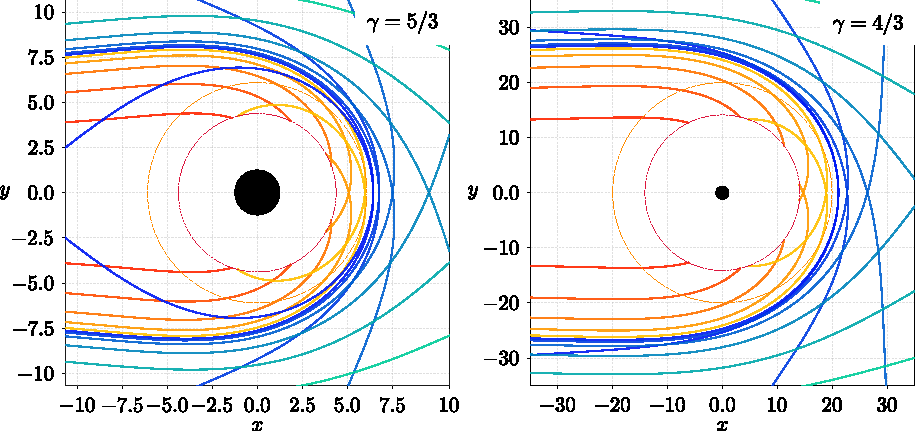
\includegraphics[width=\linewidth]{phonon_orbits_both.pdf}
\caption{Sound ray trajectories in the Michel flow at $a_{\infty}=0.1$ for a monatomic gas ($\gamma=5/3$, left) and radiation-dominated plasma ($\gamma=4/3$, right). Captured rays ($b<b_{\mathrm{c}}$) spiral onto the acoustic horizon $r_{\mathrm{a}}$, while scattered rays ($b>b_{\mathrm{c}}$) are deflected, wrapping around the acoustic photon sphere $r_{\mathrm{aph}}$.}
\label{fig:phonon-orbits}
\end{figure}

\begin{figure}[p]
\centering
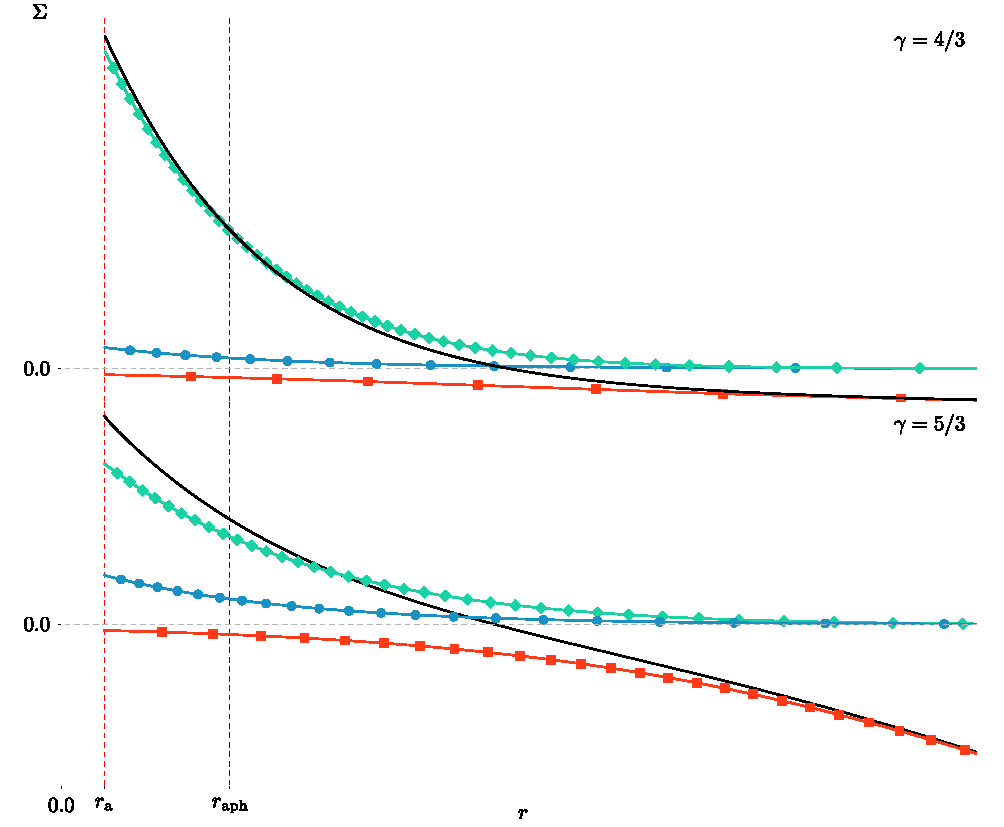
\includegraphics[width=0.8\linewidth]{phonon_forces.pdf}
\caption{Decomposition of the force~\eqref{eq:binet-second-acoustic} along the critical ray $b=b_{\mathrm{c}}$ ($a_{\infty}=0.1$) for $\gamma=4/3$ (top) and $\gamma=5/3$ (bottom).}
\label{fig:phonon-forces}
\end{figure}

\begin{figure}[p]
\centering
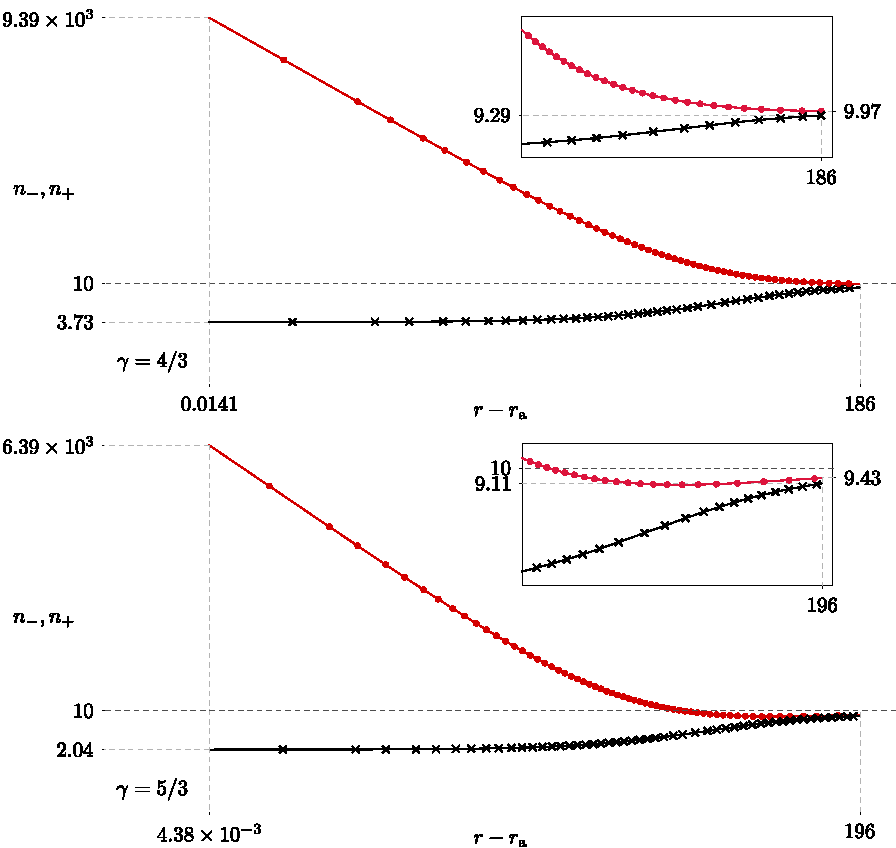
\includegraphics[width=0.75\linewidth]{shapiro_compare.pdf}
\caption{Local slowdown $n_{\pm}=f/|v_{\pm}|$ for outgoing and ingoing rays ($a_{\infty}=0.1$). Near the horizon, the outgoing branch freezes ($n_{+}\to\infty$), while the ingoing branch remains finite.}
\label{fig:shapiro}
\end{figure}

\begin{figure}[p]
\centering
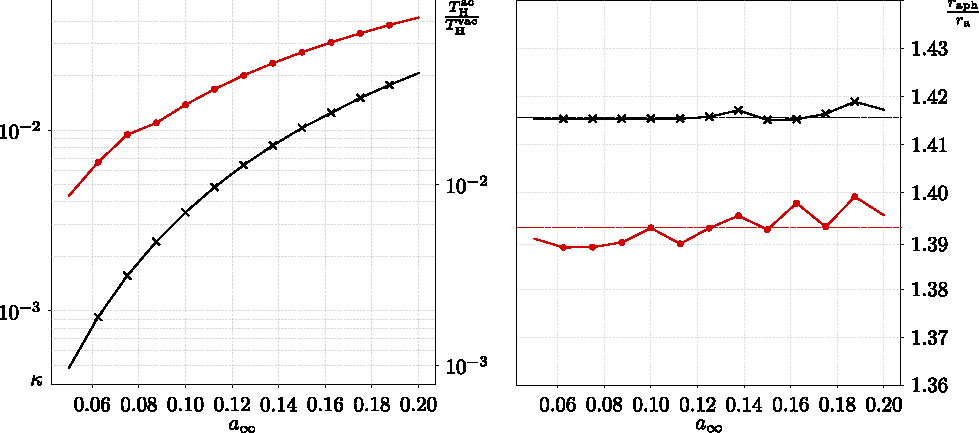
\includegraphics[width=0.88\linewidth]{ainf_scan.pdf}
\caption{Dependence of the acoustic horizon thermodynamics and lensing geometry on the asymptotic sound speed $a_{\infty}$. The ratio $r_{\mathrm{aph}}/r_{\mathrm{a}}$ remains nearly constant.}
\label{fig:ainf-scan}
\end{figure}

\clearpage
\begin{table}[p]
\centering
\caption{Michel sonic point (coinciding with the acoustic horizon), $r_{\mathrm{a}}=r_{\mathrm{c}}$, and the sound speed $a_{\mathrm{c}}$ at it.}
\label{tab:sonic-point}
{\small
\begin{tabular}{cccc}
\toprule
$\gamma$ & $a_{\infty}$ & $r_{\mathrm{a}}=r_{\mathrm{c}}$ & $a_{\mathrm{c}}$ \\
\midrule
$4/3$ & $0.01$ & $1252$ & $0.014$ \\
$4/3$ & $0.03$ & $141$  & $0.042$ \\
$4/3$ & $0.10$ & $14.1$ & $0.137$ \\
$5/3$ & $0.01$ & $38.1$ & $0.082$ \\
$5/3$ & $0.03$ & $13.1$ & $0.142$ \\
$5/3$ & $0.10$ & $4.38$ & $0.262$ \\
\bottomrule
\end{tabular}
}
\end{table}

\begin{table}[p]
\centering
\caption{Forces $F_{\mathrm{E}}$, $F_{\mathrm{R}}$, $F_{\mathrm{W}}$ from~\eqref{eq:binet-second-acoustic} and their sum $\Sigma=F_{\mathrm{E}}+F_{\mathrm{R}}-F_{\mathrm{W}}$. $a_{\infty}=0.1$.}
\label{tab:phonon-forces}
{\small
\setlength{\tabcolsep}{4.5pt}
\begin{tabular}{llcccccc}
\toprule
$\gamma$ & point & $r$ & $F_{\mathrm{E}}$ & $F_{\mathrm{R}}$ & $F_{\mathrm{W}}$ & $\Sigma$ & $1/b^{2}_{\mathrm{c}}$ \\
\midrule
\multirow{3}{*}{$5/3$}
  & $r_{\mathrm{a}}$   & $4.38$  & $+7.81\cdot 10^{-2}$ & $-8.95\cdot 10^{-3}$ & $-2.55\cdot 10^{-1}$ & $+3.24\cdot 10^{-1}$ & \multirow{3}{*}{$4.01\cdot 10^{-4}$} \\
  & $r_{\mathrm{aph}}$ & $6.10$  & $+4.04\cdot 10^{-2}$ & $-1.54\cdot 10^{-2}$ & $-1.39\cdot 10^{-1}$ & $+1.64\cdot 10^{-1}$ & \\
  & $r_{0}$          & $12.16$ & $+1.01\cdot 10^{-2}$ & $-4.49\cdot 10^{-2}$ & $-3.47\cdot 10^{-2}$ & $0$ & \\
\midrule
\multirow{3}{*}{$4/3$}
  & $r_{\mathrm{a}}$   & $14.11$ & $+7.53\cdot 10^{-3}$ & $-2.23\cdot 10^{-3}$ & $-1.15\cdot 10^{-1}$ & $+1.20\cdot 10^{-1}$ & \multirow{3}{*}{$1.73\cdot 10^{-5}$} \\
  & $r_{\mathrm{aph}}$ & $19.98$ & $+3.76\cdot 10^{-3}$ & $-3.26\cdot 10^{-3}$ & $-4.96\cdot 10^{-2}$ & $+5.01\cdot 10^{-2}$ & \\
  & $r_{0}$          & $43.41$ & $+7.96\cdot 10^{-4}$ & $-6.45\cdot 10^{-3}$ & $-5.65\cdot 10^{-3}$ & $0$ & \\
\bottomrule
\end{tabular}
}
\end{table}

\begin{table}[p]
\centering
\caption{Integral characteristics of the acoustic Shapiro effect. $a_{\infty}=0.1$.}
\label{tab:shapiro}
{\small
\setlength{\tabcolsep}{4.5pt}
\begin{tabular}{lccccccc}
\toprule
$\gamma$ & $r_{1}/r_{\mathrm{a}}$ & $r_{1}$ & $n_{+}$ & $n_{-}$ & $\Delta t^{\mathrm{ac}}_{+}$ & $R$ & $\mathcal{T}$ \\
\midrule
\multirow{3}{*}{$4/3$}
  & $1{+}10^{-3}$ & $14.1$ & $9.39\cdot 10^{3}$ & $3.73$ & $2813$ & $1035$ & $15.9$ \\
  & $1.5$         & $21.2$ & $27.2$             & $4.60$ & $1875$ & $819$  & $11.3$ \\
  & $4.0$         & $56.4$ & $11.7$             & $7.12$ & $1357$ & $1062$ & $10.4$ \\
\midrule
\multirow{3}{*}{$5/3$}
  & $1{+}10^{-3}$ & $4.39$ & $6.39\cdot 10^{3}$ & $2.04$ & $1902$ & $467$ & $10.5$ \\
  & $1.5$         & $6.57$ & $20.3$             & $2.55$ & $1663$ & $465$ & $9.42$ \\
  & $4.0$         & $17.5$ & $9.97$             & $4.34$ & $1526$ & $613$ & $9.24$ \\
\bottomrule
\end{tabular}
}
\end{table}

\begin{table}[p]
\centering
\caption{Surface gravity of the acoustic horizon from~\eqref{eq:surface-gravity-explicit}. $a_{\infty}=0.1$.}
\label{tab:surface-gravity}
{\small
\begin{tabular}{ccccc}
\toprule
$\gamma$ & $r_{\mathrm{a}}=r_{\mathrm{c}}$ & $\kappa$ & $T_{\mathrm{H}}=\kappa/2\pi$ & $2\kappa=T^{\mathrm{ac}}_{\mathrm{H}}/T^{\mathrm{vac}}_{\mathrm{H}}$ \\
\midrule
$5/3$   & $4.38$  & $1.38\cdot 10^{-2}$ & $2.20\cdot 10^{-3}$ & $2.76\cdot 10^{-2}$ \\
$4/3$   & $14.11$ & $3.51\cdot 10^{-3}$ & $5.58\cdot 10^{-4}$ & $7.02\cdot 10^{-3}$ \\
\midrule
vacuum    & $1$     & $1/2$               & $1/4\pi$            & $1$ \\
\bottomrule
\end{tabular}
}
\end{table}

\begin{table}[p]
\centering
\caption{Dependence on the asymptotic sound speed $a_{\infty}$.}
\label{tab:ainf-scan}
{\small
\begin{tabular}{ccccccc}
\toprule
$\gamma$ & $a_{\infty}$ & $r_{\mathrm{a}}$ & $r_{\mathrm{aph}}$ & $r_{\mathrm{aph}}/r_{\mathrm{a}}$ & $\kappa$ & $2\kappa$ \\
\midrule
\multirow{4}{*}{$5/3$}
  & $0.05$ & $8.13$ & $11.29$ & $1.39$ & $4.10\cdot 10^{-3}$ & $8.20\cdot 10^{-3}$ \\
  & $0.10$ & $4.38$ & $6.10$  & $1.39$ & $1.38\cdot 10^{-2}$ & $2.76\cdot 10^{-2}$ \\
  & $0.15$ & $3.14$ & $4.37$  & $1.39$ & $2.69\cdot 10^{-2}$ & $5.39\cdot 10^{-2}$ \\
  & $0.20$ & $2.51$ & $3.52$  & $1.40$ & $4.19\cdot 10^{-2}$ & $8.39\cdot 10^{-2}$ \\
\midrule
\multirow{4}{*}{$4/3$}
  & $0.05$ & $51.67$ & $73.13$ & $1.42$ & $4.82\cdot 10^{-4}$ & $9.64\cdot 10^{-4}$ \\
  & $0.10$ & $14.11$ & $19.97$ & $1.42$ & $3.51\cdot 10^{-3}$ & $7.02\cdot 10^{-3}$ \\
  & $0.15$ & $7.10$  & $10.06$ & $1.42$ & $1.03\cdot 10^{-2}$ & $2.06\cdot 10^{-2}$ \\
  & $0.20$ & $4.60$  & $6.51$  & $1.42$ & $2.06\cdot 10^{-2}$ & $4.13\cdot 10^{-2}$ \\
\bottomrule
\end{tabular}
}
\end{table}

\clearpage
\bibliographystyle{elsarticle-num}
\bibliography{article}

\end{document}